\documentclass[conference]{IEEEtran}
\usepackage{graphicx}
\usepackage{amsmath}
\usepackage{cite}
\usepackage{subcaption} % For subfigures and captions
\usepackage{caption}
\captionsetup[figure]{labelformat=simple, labelsep=period}


\title{Waypoint Generation based on Crop Row Detection Using Unet and Hough Transform}

\author{
	\IEEEauthorblockN{Alireza Amiri}
	\IEEEauthorblockA{Department of Electrical Engineering\\
		K N. Toosi University of Technology\\
		Tehran, Iran\\
		ali.amiri@email.kntu.ac.ir}
	\and
	\IEEEauthorblockN{Saeed Khankalantary}
	\IEEEauthorblockA{Department of Electrical Engineering\\
		K N. Toosi University of Technology\\
		Tehran, Iran\\
		s.kalantary@kntu.ac.ir}
}

\begin{document}
	
	\maketitle
	
	\begin{abstract}
		In autonomous agriculture, using wheeled mobile robots for various tasks requires the precise generation of waypoints to accurately define the robots' paths. This article presents a method that utilizes aerial imagery to detect crop positions and establish waypoints. In the image processing stage of this paper, crop detection was assessed using two methods of color-filtering-based and Unet-based image segmentation, with Unet outperforming with 96\%\ accuracy and 84\%\ of IoU and showing satisfying results on different fields, considering the presence of unwanted vegetation. Subsequently, two crop row detection processes, including Linear Regression and the Hough Transform, were analyzed, presenting the convenient implementation of the Hough Transform compared to linear regression while having more accurate predictions. A mathematical conversion factor was derived to convert the position of pixels selected as path points to the global coordination systems. Finally, a specialized hardware setup comprising a high-resolution camera and a radio transmission system has been developed to capture and transmit live images of the agricultural field, enabling the system to support real-time crop detection and waypoint generation. Lastly, the potential of the introduced system is discussed to be implemented in future works.
	\end{abstract}
	
	\begin{IEEEkeywords}
		Crop Row Detection, Hough Transform, Precision Agriculture, Unet, Image Processing
	\end{IEEEkeywords}
	
	\section{Introduction}
	Integrating technologies like artificial intelligence, sensing systems, and autonomous robots is vital for enhancing agricultural productivity and sustainability amid global food challenges \cite{b2,b3}. Precision Agriculture (PA) optimizes resource use—such as water and fertilizers—based on site-specific requirements, improving crop yields and minimizing environmental impacts \cite{b5,b6}. Consequently, mobile robots are increasingly used for tasks like fertilization, irrigation, and harvesting \cite{b2,b3}.
	
	Despite the widespread use of GPS-based path planning in PA, issues like crop damage from misalignment with rows persist \cite{b1}. Machine vision-based detection is gaining traction for precise, real-time path planning, reducing crop injury \cite{b1,b8}. However, the unstructured nature of agricultural environments complicates navigation. Robotic systems incorporate sensors such as scanning lasers and machine vision cameras to tackle this issue. \cite{b2,b3}, while UAVs provide high-resolution aerial sensing, overcoming the limitations of ground-based platforms \cite{b10}.
	
	UAVs are essential in PA, offering versatile remote sensing capabilities \cite{b9,b12}. They provide valuable data for monitoring crop variability and support temporal and spatial analyses \cite{b10,b12}. Applications in vegetation segmentation, crop row detection, and ground-based sensing gaps are examples of their usage \cite{b7,b13}. Despite challenges like limited flight endurance, UAVs' ability for autonomous flights and timely data collection make them crucial in modern agriculture \cite{b11,b13}. Nevertheless, incorporating aerial imagery into precision farming requires advanced post-processing to distinguish crop rows from soil and weeds accurately \cite{b6}.
	
	Crop row detection methods utilize various approaches to enhance precision in agricultural applications. Techniques such as vegetation indices (NDVI, ExG, SAVI), along with thresholding, clustering, and the Minimum Distance to the Mean (MDM) classifier, effectively segment vegetation from soil \cite{b1,b6,b13}. Fusion methods that combine RGB and NDVI data further improve segmentation for autonomous navigation \cite{b5}.
	
	AI-based approaches, particularly deep learning models, have recently advanced detection accuracy. For example, CRowNet—a model combining convolutional neural networks (CNNs) with the Hough Transform—demonstrates high detection rates in complex scenarios \cite{b8,b14}. Additionally, architectures like U-Net, SegNet, and ModSegNet often outperform classical methods in challenging environments \cite{b5,b13}.
	
	Traditional computer vision techniques like the Hough Transform remain relevant despite challenges like computational complexity and noise sensitivity \cite{b2,b15}. Adaptations like the Probabilistic and Multi-scale Hough Transforms enhance efficiency and accuracy \cite{b2}. Combining these with deep learning improves detection capabilities \cite{b8}. Other methods, including linear regression and Blob Analysis, contribute, albeit with specific limitations depending on field conditions \cite{b2,b3}. Machine learning models like Faster R-CNN and YOLOv3 enhance row detection accuracy \cite{b2,b5}.
	
	Information extracted from crop rows is essential in precision agriculture, supporting tasks like guiding autonomous vehicles and generating vigor maps for field partitioning. In aerial imagery, navigation paths are defined by lines between crop rows, while ground-based vehicles utilize the central angle between rows for path planning \cite{b11,b1}.
	
	
	
	This paper presents a novel system for precise navigation in autonomous agricultural robots through real-time aerial image acquisition and waypoint generation. The system integrates a quadcopter-mounted camera and a radio transmission system to capture and relay high-resolution RGB images and GPS coordinates. Aerial images are divided into sub-images and processed using color filtering and a UNet model for crop detection. Crop row detection is refined via linear regression and the Hough Transform, and waypoints are generated by mapping pixel data to GPS coordinates. 
	
	Key contributions include: 
	
	\begin{itemize}
		
		\item \textbf{Design and implementation of the image processing pipeline} for image segmentation using Unet and crop row detection using Hough transform.
		\item \textbf{Derive a mathematical conversion factor} for converting pixel positions to global coordination.
		\item \textbf{Develop an experimental setup} for live aerial image and GPS signal data acquisition.
	\end{itemize}
	
	This approach enhances the navigation capabilities of agricultural robots in complex environments.
	
	The rest of this paper is structured as follows. Section \ref{Data Acquisition} introduces a hardware setup for aerial imagery data acquisition. Section \ref{Image Processing} explains the image processing procedure, including image splitting, applying two methods—K-means clustering and the U-Net model—for image segmentation, crop row detection using linear regression and Hough Transform, and the waypoint generation method. The section concludes with the reconstruction of split images. Section \ref{Waypoint Generation} introduces a conversion factor to convert the local position of waypoints obtained by previous sections to the global coordinate system. The experimental setup of the proposed system is presented in \ref{Experimental Setup}. The results achieved by developed systems are presented in \ref{Results and Discussion}. Conclusions and further improvements are finally discussed in
	\ref{Conclusion}.
	
	\section{Methodology}
	
	This section outlines the procedures for generating waypoints in agricultural fields using aerial imagery. The process commenced with capturing high-resolution images, which underwent several steps, including image segmentation, to distinguish crops from the background. Two methods—linear regression and Hough Transform—were employed to detect crop rows and assess their layout. Subsequently, waypoints were generated along the paths between the rows. Finally, a pixel-to-meter conversion was performed to transform local waypoint coordinates into global coordinates, ensuring accurate spatial mapping. Fig. \ref{fig_procedure} illustrates the proposed procedure.
	
	
	\begin{figure}[t]
		\includegraphics[width=\linewidth]{Block Diagram.png}
		\caption{procedure of waypoint generation using aerial images
			\cite{b5}}
		\label{fig_procedure}
	\end{figure}
	
	\subsection{Data Acquisition}\label{Data Acquisition}
	In order to facilitate the real-time generation of waypoints in agricultural fields, a robust hardware setup is essential for capturing and transmitting environmental data to the processing unit. A lightweight camera is critical for obtaining high-resolution aerial images of the target field, serving as the primary data source for the image processing algorithm. Several cameras, including Sequoia \cite{b9,b4,b7,b6}, Micasense RedEdge \cite{b9,b14}, and DJI Zenmuse X7 \cite{b5}, have been employed in similar projects. High-resolution RGB images were deemed sufficient for this project based on the specifications of these cameras and the requirements of crop row detection algorithms. While the NIR band offers valuable insights for vegetation segmentation, its sensitivity to environmental conditions, such as temperature, can adversely affect software performance \cite{b5}. 
	
	Consequently, the GoPro HERO4 camera was selected for this project due to its lightweight design, high-quality RGB imaging, and durability. Figure \ref{gopro} illustrates the camera used in this research. A radio transmission system comprising power supplies, a transmitter, and a receiver was developed to enable live data transfer from the quadcopter-mounted camera to the image processing software. 
	
	Lastly, converting pixel coordinates from images to global coordinates necessitates the camera's global position during image capture. Therefore, a Ublox Neo-6m GPS module was mounted on the quadcopter to provide this reference information.
	
	
	\begin{figure}[t]
		\centering
		\includegraphics[width=0.7\linewidth]{GoPro.jpg}
		\caption{GoPro camera used in this paper}
		\label{gopro}
	\end{figure}
	
	
	\subsection{Image Processing}\label{Image Processing}
	The main contribution of this paper lies in this section, which is to develop an image-processing pipeline to determine the position of pixels in the path between the crops. Fig.
	\ref{fig_procedure}
	shows the procedure proposed in this paper. Initially, the aerial images captured with the camera are split into sub-images. Then, during a semantic segmentation process, a binary mask is generated for each sub-image showing the positions of vegetation and background. In the next step, using Hough Transform, crop rows are detected. After defining the path line, a desired number of equally spaced points are selected on this line, and their position is recorded for later steps. Finally, the sub-images and their local waypoint coordinates are reconstructed, forming the original input image.
	
	\subsubsection{Preprocessing}\label{Preprocessing}\leavevmode
	
	High-resolution aerial images covering large areas are typically too large to be used directly in image processing algorithms and networks.
	Besides, due to the variation in terrain topologies, the non-uniform shape of crop rows -including curved or irregular shapes- is common in some agricultural fields
	\cite{b2, b3, b14}.
	Fig. \ref{fig_Aerial} shows an example of aerial images used in similar projects.
	Given this information, calculating a straight line for an entire crop row in the original image is not an accurate approach for crop row detection.
	To address this issue, the aerial image is initially split into equal-sized sections with a static image size of 512 by 512 pixels. These sub-images are named accordingly and will be reconstructed after the image-processing procedure. Their chosen size ensures compatibility with the algorithms and networks designed in the later steps of the image-processing section.
	
	
	\begin{figure}[t]
		\centering
		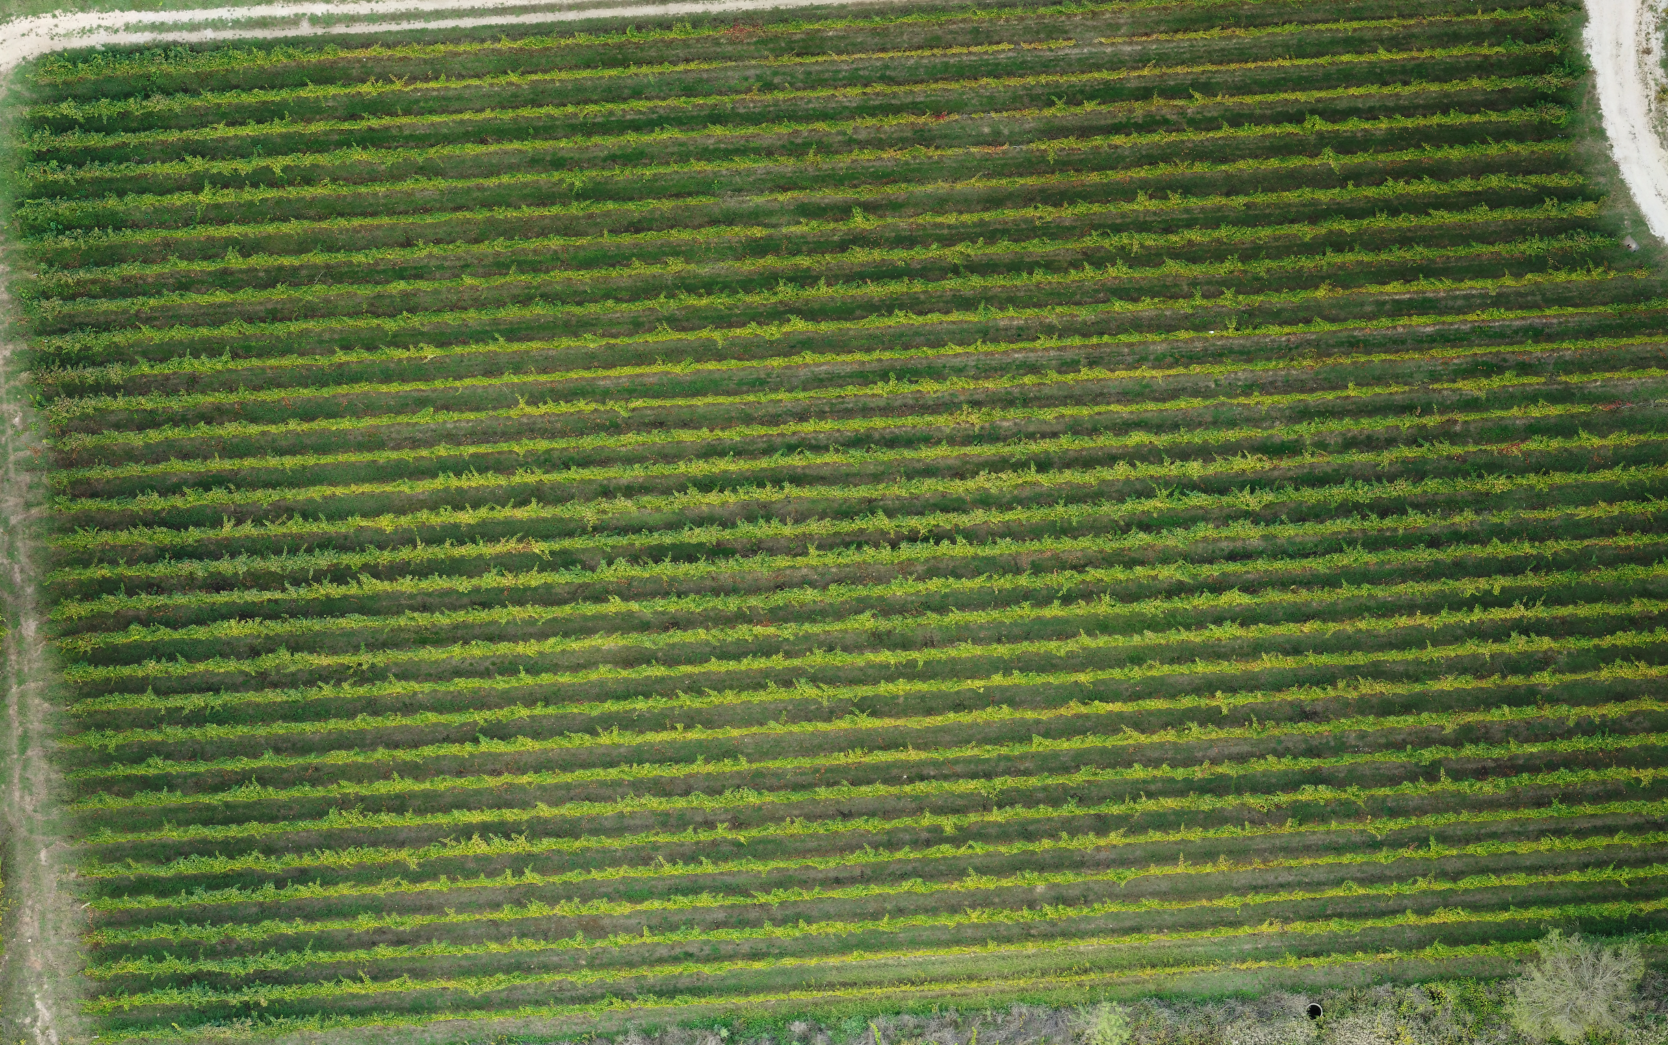
\includegraphics[width=0.7\linewidth]{Aerial Image2.png}
		\caption{Aerial image sample used for waypoint detection
			\cite{b5}}
		\label{fig_Aerial}
	\end{figure}
	
	\subsubsection{Image Segmentation}\label{Image Segmentation}\leavevmode
	
	Image segmentation is this project's most computationally intensive section, and its outcome directly impacts the system's overall accuracy. Given the RGB sub-images, it is essential to identify the exact locations where crops exist, which is done by processing the image and generating a binary mask. The following section introduces and implements two semantic segmentation methods, and their results are assessed.
	
	\paragraph{Color-Filtering Based Image Segmentation}\leavevmode
	
	The initial idea for image segmentation of crops in agricultural fields was to apply color filtering methods to isolate the areas having a green color. This method was first used by analyzing the image's green channel but performed poorly for a few reasons. First, the green channel filtering method cannot filter white pixels since they also include a large amount of green color. Second, there are sections of crops with color tending to yellow, which were unintentionally removed from the layer mask. The two issues mentioned were later resolved using a prefiltering for white pixels removal and also by converting the RGB image to HSV format (Hue, Saturation, and Value) so that it would be possible to filter the pixels based on their color considering their Vegetation Index (VI).
	
	Next, a K-means clustering method was applied to the color-based filtered image to highlight the areas, including crops. The clustering helped remove sparse pixels identified as crops and unite the areas where crops exist. The Parameters of the K-means algorithm were defined in an iterative approach to determine the best-performing setting,
	
	
	\paragraph{Unet-Based Image Segmentation}\leavevmode
	
	The limited performance of color-based image segmentation in crop fields indicates the need for an intelligent model that can recognize the crops using more complicated methods. Utilizing machine learning methods to train semantic segmentation models has proven to be a reliable solution for crop detection. This approach chose a Unet network as the primary image segmentation tool (See Fig.
	\ref{fig_Unet})
	and was trained on a dataset developed by
	\cite{b5}
	.This dataset consists of quadcopter-based aerial images taken from three vineyards with corresponding ground truth images, indicating the location of vines in the vineyard.
	
	The original and ground truth images were initially split into sub-images using a sliding window of size 512 by 512 pixels to use the annotated aerial images. The sliding step size was chosen to be 50 pixels, which resulted in more sample data for training. The resulting dataset consists of 5089 sub-images, which are divided into train, test, and validation sets with a ratio of 80\%\
	, 10\%\
	, 10\%\
	.
	
	
	\begin{figure}[t]
		\includegraphics[width=\linewidth]{UNET.png}
		\caption{Unet model architecture}
		\label{fig_Unet}
	\end{figure}
	
	\subsubsection{Crop Row Detection}\label{Crop Row Detection}\leavevmode
	
	The crop row detection process aims to assign a straight line with a defined slope and intercept each group of white pixels annotated as crops in the binary mask. This study analyzed and implemented two approaches—linear regression and the Hough Transform—for this purpose.
	
	\paragraph{Linear Regression}\label{Linear Regression}\leavevmode
	
	This experiment used the binary layer mask of segmented crops to assign each pixel to its corresponding crop row. The process began by determining the optimal angle of the crop rows using an iterative algorithm, assuming all rows were parallel with the same slope. Once the slope was defined, the x and y coordinates of the white pixels were rotated to align the crop rows vertically, simplifying clustering.
	
	Next, the K-means algorithm was applied with a customized loss function, which, unlike traditional loss functions centered around a point, minimizes the least square error between the white pixels and a vertical line. 
	
	Due to the variability in the number of clusters across images, the algorithm started by grouping nearby pixels and designating isolated pixels as new cluster centers. However, this led to the formation of several unwanted clusters. To resolve this, adjacent clusters were merged. Finally, the pixel coordinates were rotated back to visualize the clusters, and linear regression was used to fit a line to the pixels within each cluster.
	
	
	\paragraph{Hough Transform}\label{Hough Transform}\leavevmode
	
	Another widely used solution for crop row detection is the Hough Transform. This computer vision technique is primarily designed to identify geometric shapes in images, making it particularly effective for detecting lines and curves. In this project, the Hough Transform was employed as an alternative to the linear regression model for predicting crop rows. Implementing this method requires significantly less preprocessing and image manipulation, mainly due to the availability of related packages in OpenCV.
	
	\subsubsection{Path Waypoint Generation}\label{Path Waypoint Generation}\leavevmode
	
	As stated in previous steps, the most computational parts of this study are image segmentation and crop row detection. Determining crop rows as lines with defined slope and intercept makes calculating a line indicating the path straightforward. The path is defined as a line parallel to two neighboring crop rows at an equal distance from each other.
	Waypoints can be defined by choosing a specific number of equally spaced points along each path. The local coordination of these waypoints is stored for later study steps.
	
	\subsubsection{Reconstruction of Aerial Image}\label{Reconstruction of Aerial Image}\leavevmode
	
	Following the image splitting described in the section
	\ref{Preprocessing}, the image processing tasks outlined earlier will be applied to each segment of the leading aerial image. The goal is to determine and record the waypoint coordinates within each segment. Once the waypoint coordinates are computed, the initial image must be reconstructed and assembled. Subsequently, the waypoint coordinates need to be converted to align with the coordinates of the newly assembled image.
	
	\subsection{Waypoint Generation}\label{Waypoint Generation}
	An analytical approach and mathematical algorithm are required to obtain the corresponding global coordinates of the points identified in the images. This process involves using the global coordinates of the camera at the time of image capture, along with the camera's height.
	
	\begin{figure}[t]
		\centering
		\includegraphics[width=0.6\linewidth]{waypoint_geometry}
		\caption{Geometrical representation of waypoint generation}
		\label{fig:waypointgeometry}
	\end{figure}
	
	Assuming the camera is positioned at the center of the image at a height of \( h \), and given the angle \( \theta \) (See Fig. \ref{fig:waypointgeometry}), the conversion of pixel position to distance is described by the following equations:
	\begin{equation}
		\tan \theta = \frac{x}{h} \implies x = \tan \theta  \cdot h
		\label{eq:1}
	\end{equation}
	
	Where \( x \) is the distance from the camera position to the image's edge in meters.
	
	Assuming the image to be in a square frame and the resolution is \( L \) by \( L \) pixels, then:
	
	\begin{equation}
		{x}=\frac{L}{2}\left(pixel\right)
		\label{eq:2}
	\end{equation}
	
	using Eq.\ref{eq:1} and Eq.\ref{eq:2} implies:
	
	\begin{equation}
		1 \text{ (pixel)} = 2h \cdot \frac{\tan \theta}{L} \text{ (m)}
		\label{eq:3}
	\end{equation}
	
	
	Achieving Eq.\ref{eq:3}, the actual distance between the position of the quadcopter and any point on the ground corresponding to coordination \((x, y)\) in the image can be calculated. 
	
	To generate the waypoints, which are in the form of latitude and longitude, a conversion factor of meter to global coordination is required, which is shown in Eq.\ref{eq:4} 
	
	\begin{equation}
		1 \text{ (m)} = 0.00001^\circ
		\label{eq:4}
	\end{equation}
	
	Thus, using Eq.\ref{eq:3} and Eq.\ref{eq:4} implies the final conversion factor for calculation of the change in global coordination as defined in Eq. \ref{eq:5}:
	
	\begin{equation}
		1 \text{ (pixel)} = 0.00002 \times h \cdot \frac{\tan \theta}{L}^\circ
		\label{eq:5}
	\end{equation}
	
	Lastly, the relative change in global coordinates is added to the quadcopter's GPS-derived coordinates along the latitude and longitude axes to generate waypoints and obtain accurate global pixel coordinates.
	
	
	\section{Experimental Setup}\label{Experimental Setup}
	In alignment with the primary objective of this research, which aimed to develop an integrated system for acquiring live aerial imagery and calculating global coordinates for path waypoints, an experimental setup incorporating a camera and radio transmission system was designed and implemented. Using the RC805 radio transmission system, a wireless connection between the camera and a computer was established to facilitate the transfer of live images captured by a GoPro Hero4 camera. The experimental configuration is illustrated in Fig.
	\ref{EXP}.
	
	The previously described image processing features were consolidated into a program with a graphical user interface (GUI). This system allows for two modes of operation: offline, where pre-existing images stored locally on the computer are loaded, and online, where live-stream imagery from the camera is received. The results of each image processing step are subsequently displayed in the program's output, providing a visual representation of the logic underpinning the generated waypoints.
	
	
	
	
	\begin{figure}[t]
		\includegraphics[width=\linewidth]{Setup of experiment.png}
		\caption{Experimental setup of proposed waypoint generation system}
		\label{EXP}
	\end{figure}
	
	\section{Results and Discussion}\label{Results and Discussion}
	
	This section evaluates the performance of the methods mentioned earlier and presents the visual and statistical outputs of the image processing algorithms, including semantic segmentation and crop row detection. Subsequently, the results obtained from the experimental setup in waypoint generation are analyzed and discussed.
	\subsection{Image Segmentation}
	
	The Color-filtering-based image segmentation method demonstrated the ability to produce an accurate binary mask indicating vegetation presence without high computational costs. However, the method exhibited limitations when applied to images from diverse fields with various crops. Due to its reliance on color filtering, it could not differentiate between crops and unwanted vegetation, such as grass and weeds. This issue aligns with observations reported in \cite{b5}, as illustrated in Fig.
	\ref{fig2:kmeans}.
	
	
	In contrast, the Unet-based segmentation method, trained over 50 epochs, reached an early stopping criterion at epoch 7, achieving an accuracy of 96\%\, IoU of 84\%\, F1 score of 0.91 and a loss of 0.09. The F1 score of the proposed method outperforms the mean measure of the corresponding test in \cite{b5}, which was reported as 0.77. The model effectively segmented crops under different conditions, even when unwanted vegetation was present, as demonstrated in Fig.
	\ref{fig2:Unet_Segmentation}.
	This highlights its robustness compared to the Color-Filtering method.
	
	\begin{figure}[t]
		\begin{subfigure}{\linewidth}
			\centering
			\includegraphics[width=0.7\linewidth]{kmeans_predictions.png}
			\caption{Color-Filtering Based Image Segmentation}
			\label{fig2:kmeans}
		\end{subfigure}
		
		\vspace{0.5cm}
		
		\begin{subfigure}{\linewidth}
			\centering
			\includegraphics[width=0.7\linewidth]{unet_predictions.png}
			\caption{Unet-Based Image Segmentation}
			\label{fig2:Unet_Segmentation}
		\end{subfigure}
		
		\caption{Image Segmentation Results \cite{b5}}
		\label{fig:Image_Segmentation_Results}
	\end{figure}
	
	\subsection{Crop Row Detection}
	
	In implementing crop row detection, the linear regression approach proved ineffective. The method's complexity and computational intensity yielded unsatisfactory results, prompting exploring alternative techniques.(See Fig.\ref{fig_Linear_Regression})
	
	In contrast, the Hough Transform method achieved satisfactory results with less computational overhead. Due to the availability of relevant packages in OpenCV, this method required minimal preprocessing. Upon application, the Hough Transform successfully detected multiple lines for each crop row, as shown in Fig. 
	\ref{fig_Hough_Init}
	. To refine these results, the detected lines were merged, and a single line per crop row was determined by averaging the slope and intercept values. The final output, displayed in Fig. 
	\ref{fig_Hough_mod} demonstrates the effectiveness of this approach for accurate crop row detection.
	
	\begin{figure}[t]
		\centering
		\begin{subfigure}{\linewidth}
			\centering
			\includegraphics[width=0.5\linewidth]{Kmeans_Row_Result.png}
			\caption{Linear regression based crop row detection}
			\label{fig_Linear_Regression}
		\end{subfigure}
		
		\vspace{0.5cm}
		
		\begin{subfigure}{\linewidth}
			\centering
			\includegraphics[width=0.7\linewidth]{Hough initial2.png}
			\caption{Initial Hough transform implementation}
			\label{fig_Hough_Init}
		\end{subfigure}
		
		\vspace{0.5cm} % Adjust the space between the two subfigures as needed
		
		\begin{subfigure}{\linewidth}
			\centering
			\includegraphics[width=0.7\linewidth]{Hough Revised2.png}
			\caption{Modified Hough transform implementation}
			\label{fig_Hough_mod}
		\end{subfigure}
		
		\caption{Crop row detection methods using Hough transform \cite{b5}}
		\label{fig:comparison}
	\end{figure}
	
	\subsection{Waypoint Generation}
	
	The waypoint generation system, combined with the hardware setup, successfully captured live aerial imagery using a quadcopter-mounted camera and transmitted these to a ground-based receiver via a radio transmission system. The experimental setup confirmed the feasibility of image transmission over varying distances to the processing unit, demonstrating the system’s potential for real-time data acquisition.
	
	The waypoint generation component also effectively converted local pixel positions within the images to global coordinates. The transformation described in Eq.\ref{eq:5} produced accurate global pixel coordinates and integrated with the quadcopter’s GPS data along the latitude and longitude axes, facilitating precise waypoint generation.
	
	However, the system has yet to be tested in operational field environments. Therefore, while preliminary results are promising, further field experiments are necessary to validate the system’s performance under practical conditions. Future work will focus on fully implementing and assessing the image transmission and waypoint generation processes to ensure their robustness and reliability in real-world applications.
	
	
	\section{Conclusion}\label{Conclusion}
	This paper proposed a solution for precise navigation in autonomous agricultural robots, focusing on a hardware setup and image processing pipeline for acquiring live aerial images and identifying global waypoints within agricultural fields. A feasibility study demonstrated the potential of using a quadcopter-mounted camera, GPS, and a radio transmission system to capture and transmit high-resolution RGB images in real-time.
	
	Two image segmentation methods—Color-Filtering and Unet-based—were evaluated. While the Color-Filtering method proved ineffective in the presence of unwanted vegetation, the Unet-based model demonstrated superior performance, achieving 96\%\ accuracy in segmenting crops, making it the preferred method.
	
	The Hough Transform outperformed the more complex linear regression approach for crop row detection, providing accurate row detection and forming the basis for defining waypoints. The final waypoints were calculated by mapping local pixel positions to global coordinates, integrating the quadcopter's GPS data, and providing reliable navigation references for agricultural robots.
	
	Although the system's feasibility was established through controlled experiments, full implementation and testing in operational field environments remain for future work.
	
	
	\begin{thebibliography}{00}
		\bibitem{b1} Y. Yang et al., "Real-time detection of crop rows in maize fields based on autonomous extraction of ROI," Expert Systems with Applications, vol. 213, p. 118826, 2023.
		\bibitem{b2} J. Shi, Y. Bai, Z. Diao, J. Zhou, X. Yao, and B. Zhang, "Row detection BASED navigation and guidance for agricultural robots and autonomous vehicles in row-crop fields: methods and applications," Agronomy, vol. 13, no. 7, p. 1780, 2023.
		\bibitem{b3} V. R. Ponnambalam, M. Bakken, R. J. Moore, J. Glenn Omholt Gjevestad, and P. Johan From, "Autonomous crop row guidance using adaptive multi-roi in strawberry fields," Sensors, vol. 20, no. 18, p. 5249, 2020.
		\bibitem{b4} N. Cunha, T. Barros, M. Reis, T. Marta, C. Premebida, and U. J. Nunes, "Multispectral image segmentation in agriculture: A comprehensive study on fusion approaches," in Iberian Robotics conference, 2023: Springer, pp. 311-323.
		\bibitem{b5} T. Barros et al., "Multispectral vineyard segmentation: A deep learning comparison study," Computers and electronics in agriculture, vol. 195, p. 106782, 2022.
		\bibitem{b6} G. Ronchetti, A. Mayer, A. Facchi, B. Ortuani, and G. Sona, "Crop row detection through UAV surveys to optimize on-farm irrigation management," Remote Sensing, vol. 12, no. 12, p. 1967, 2020.
		\bibitem{b7} M. Hassanein, M. Khedr, and N. El-Sheimy, "Crop row detection procedure using low-cost UAV imagery system," The International Archives of the Photogrammetry, Remote Sensing and Spatial Information Sciences, vol. 42, pp. 349-356, 2019.
		\bibitem{b8} M. D. Bah, A. Hafiane, and R. Canals, "CRowNet: Deep network for crop row detection in UAV images," IEEE Access, vol. 8, pp. 5189-5200, 2019.
		\bibitem{b9} I. Sa et al., "WeedMap: A large-scale semantic weed mapping framework using aerial multispectral imaging and deep neural network for precision farming," Remote Sensing, vol. 10, no. 9, p. 1423, 2018.
		\bibitem{b10} S. Sankaran et al., "Low-altitude, high-resolution aerial imaging systems for row and field crop phenotyping: A review," European Journal of Agronomy, vol. 70, pp. 112-123, 2015.
		\bibitem{b11} L. Comba, P. Gay, J. Primicerio, and D. R. Aimonino, "Vineyard detection from unmanned aerial systems images," Computers and Electronics in Agriculture, vol. 114, pp. 78-87, 2015.
		\bibitem{b12} K. Ramesh, N. Chandrika, S. Omkar, M. Meenavathi, and V. Rekha, "Detection of rows in agricultural crop images acquired by remote sensing from a UAV," International Journal of Image, Graphics and Signal Processing, vol. 8, no. 11, p. 25, 2016.
		\bibitem{b13} M. Pérez-Ortiz, J. Peña, P. A. Gutiérrez, J. Torres-Sánchez, C. Hervás-Martínez, and F. López-Granados, "A semi-supervised system for weed mapping in sunflower crops using unmanned aerial vehicles and a crop row detection method," Applied Soft Computing, vol. 37, pp. 533-544, 2015.
		\bibitem{b14} Y. Pang et al., "Improved crop row detection with deep neural network for early-season maize stand count in UAV imagery," Computers and Electronics in Agriculture, vol. 178, p. 105766, 2020.
		\bibitem{b15} N. Samet, S. Hicsonmez, and E. Akbas, "Houghnet: Integrating near and long-range evidence for bottom-up object detection," in Computer Vision–ECCV 2020: 16th European Conference, Glasgow, UK, August 23–28, 2020, Proceedings, Part XXV 16, 2020: Springer, pp. 406-423.
		\bibitem{b16} F.-A. Moreno, J. Monroy, J.-R. Ruiz-Sarmiento, C. Galindo, and J. Gonzalez-Jimenez, "Automatic waypoint generation to improve robot navigation through narrow spaces," Sensors, vol. 20, no. 1, p. 240, 2019.
	\end{thebibliography}
	
	\vspace{12pt}
	
	
\end{document}
